\documentclass[10pt,conference,compsocconf]{IEEEtran}

%\usepackage{times}
%\usepackage{balance}
\usepackage{url}
\usepackage{graphicx}
\usepackage{hyperref}
\usepackage{color}

\newcommand{\todo}[1]{}
\renewcommand{\todo}[1]{{\color{red} TODO: {#1}}}

\newcommand{\pisch}[1]{\textit{\textcolor{blue}{pisch: #1}}}

\begin{document}
\title{CIL 2018: Text Sentiment Classification}

\author{
  Aryaman Fasciati, Nikolas G\"obel, Philip Junker, Pirmin Schmid\\
  The Optimists\\
  Department of Computer Science, ETH Zurich, Switzerland
}

\maketitle

\begin{abstract}
  In this work we consider the task of classifying tweets by
  sentiment. In particular we want to determine whether a given tweet
  is associated with a positive smiley ``:)'' or a negative smiley ``:(''
  after having been stripped of these emoticons. We present two baseline models,
  a random forest classifier and a simple stacked GRU/RNN model, and a
  third more complex neural network combining GRU/RNN with convolutional
  layers and deeper NN. We trained these models on GloVe word embeddings, pre-trained
  on 2.5 billion tweets. 
  Two baselines were implemented as a reference for the prediction accuracy of our final model. 
  Our first baseline (random forest) achieved an accuracy of 72\% based on the initial first half of the test set. 
  Our second baseline (RNN/GRU) achieved an accuracy of 85.2\%.
  Our best final model achieved an accuracy of 87.4\% with this test set. After the submission deadline, an accuracy of 
  86.6\% was revealed for our model based on the second half of the test set
  that was secret during development.
\end{abstract}

\section{Introduction}

The global prevalence of social media has enabled a massive amount of users
to publicly voice their opinions and interact with each other.
Microblogging services like Twitter\footnote{\url{www.twitter.com}} make it
very easy for users to comment on current events, tell other users about their
lives, and discuss the products and services they use.
This data can be analysed for sentiments and opinions and can be used for
various purposes, such as consumer insight \cite{Chamlertwat2012}
or stock market prediction \cite{Rao:2012}.

The goal of this project is to build a sentiment classifier that
predicts whether a Twitter tweet used to include a positive smiley :) or
a negative smiley :(, based on the remaining text.

\section{Related Work}

Recurrent neural networks (RNN) with their applicability to
sequence-to-sequence (seq2seq) tasks have been used across many tasks,
especially in the natural language processing (NLP) domain, such as generating text \cite{Sutskever}.
Although RNNs seem to be primarily used for problems more
complex than binary classification, we were interested in exploring
the application of short-term memory to our task. 
Because the sentiment of a sentence often depends on more than one word 
we assumed that this will lead to a better sentiment prediction of our model.
This can be achieved via the Long short-term memory (LSTM) or 
Gated recurrent unit (GRU) variants of RNNs. Both have found extensive use in practical
applications, such as predictive chat replies \cite{allo},
question answering \cite{DiWang}, and video to text \cite{DBLP}.

\section{Models}

\subsection{First Baseline (B1)} \label{subsec:b1}

Our first baseline uses a random forest model with unlimited
max\_depth and 20 estimators. We used the random forest implementation
provided with the scikit-learn library \cite{scikit-learn}.

Tweets from the datasets are run through a pre-processing script,
provided by the GloVe project. The pre-processor normalizes tweets,
for example by replacing user names with a single token indicating a
mention. More importantly, symbols used commonly in tweets, such as
the heart ``\textless3'', are converted into tokens that are contained in the
vocabulary.

Input tweets are then split into words. Each word is looked up in the
embedding dictionary. We use 200 dimensional word embedding vectors. Words that
are not in the vocabulary are ignored. All word embeddings for a given
tweet are then aggregated into a single vector, by computing their
mean. Word embeddings are provided by the GloVe \cite{glove} project
from Stanford, pre-trained on two billion tweets.

The classifier is then trained on these tweet embeddings. We expected
this relatively simple approach to already perform quite well, because
a small number of features of single words would seem to have an
impact on overall tweet sentiment in practice. Still, aggregating word
embeddings destroys a lot of information contained in the order of
words. In particular, this approach does not differentiate between
permutations of similar words at all. It also assigns equal weight to
every word when computing the mean, whereas we would commonly expect a
small subset of words to be disproportionally strong indicators of
sentiment (``love'', ``hate'', ``good'', ``bad'', etc...).

This model achieved an accuracy of 72\% with the initial half of the test set.

\subsection{Second Baseline (B2)} \label{subsec:b2}

For the second baseline, we trained a stacked, recurrent neural
network. Two GRU cells were stacked; a hidden state size of 384 was used.
In contrast to the random forest baseline, tweet embeddings
were not aggregated in any way from their words. Rather, the network
was trained on matrices of dimension \(word\_count_{tweet} \times 200\).
Words not known in the embedding vocabulary were ignored.
Statistical analysis of the provided data in \autoref{fig:wordcount} shows that
the majority ($>$98\%) of tweets have less or equal than 30 words.
Tweets longer than that were ignored during training and shortened for prediction,
whereas shorter tweets were padded.

All output of the RNN was used as input of a single layer fully connected NN
to 2 nodes with a sigmoid activation function.
Argmax was used to determine the sentiment.
Loss was calculated with sparse softmax cross entropy with logits and
an Adam optimizer was used for learning with clipped gradient at 10
and a learning rate of $10^{-4}$.
In total, the model was trained for 4 epochs on the Leonhard cluster.
98\% of the training data was used for training; 2\% was used for evaluation.

Smaller and larger hidden state sizes were tested but resulted in
lower accuracy. Fewer (one) and more (three) layers also resulted in lower accuracy.
Additonally, we experimented with LSTM cells, which did not result in
a higher score than with GRU cells.
All outputs of the RNN were used as input of the NN to bring more state
information into the final classifier step. Using only the final hidden
state was tested and gave lower accuracy.

Typically, a matrix multiplication (and optionally addition of a bias vector) is used to
transform the output state of each RNN time step into e.g. the vocabulary space
for seq2seq predictions. Here we used the above-mentioned single-layer
fully-connected NN for the reduction from the quite large RNN output state to
the two nodes representing the sentiments, to allow for additional
non-linear transformations.

We expected this RNN model to perform better than baseline B1 because
much more implicit information could be used for the model, such as
specific word vectors and sequences of these vectors.

Indeed, this baseline model B2 achieved an accuracy of 85.2\% with the
initial half of the test set.

\begin{figure}[h!]
  \centering
  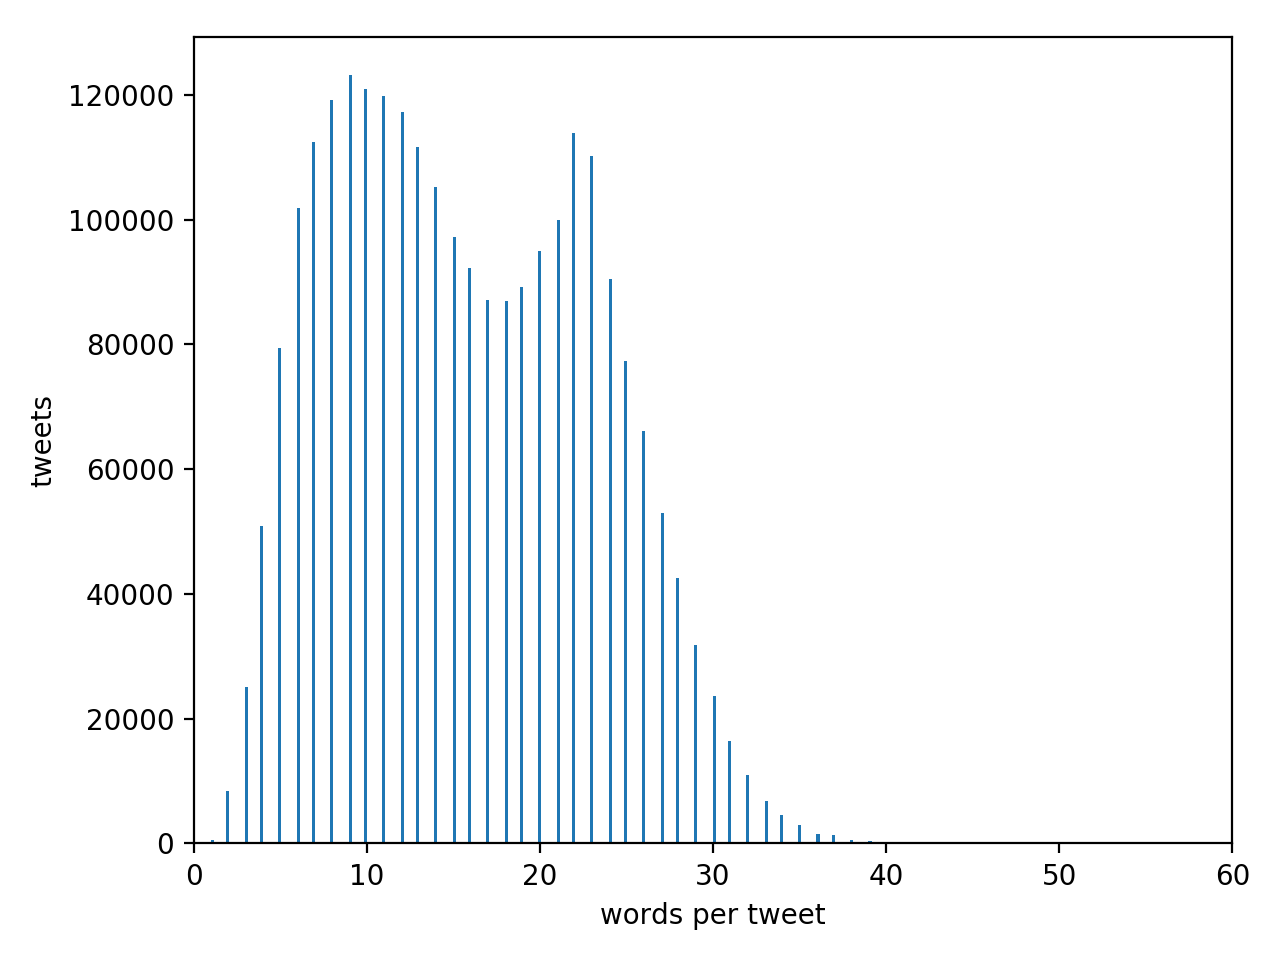
\includegraphics[scale=0.53]{word_count_histogram.png}
  \caption{Word Count Distribution}
  \label{fig:wordcount}
\end{figure}


\subsection{RNN + Convolution} \label{subsec:our-model}

With this large jump of accuracy from B1 to B2, we were very hopeful to
achieve significant improvements when adding additional
creative approaches to the problem. The most important ones are listed
in \autoref{sec:other} in more detail.

Unfortunately, most of them revealed to be unsuccessful. Thus, we settled on the
 improved model as described in detail in this section. It provided the best
 accuracy of all tested models. 

Our final model is based on the promising RNN model used in baseline B2.
We can consider the RNN output to
represent learned tweet features, which bear significance for
sentiment classification. Consequently, we wanted to re-combine these
features in a structure-preserving, context-sensitive
manner. Convolutional neural networks (CNN) fit this bill and in addition
possess the property of being invariant w.r.t
translation \cite{cnn_invariance}.
Intuitively, this sounded useful to the task at hand,
because we expect certain word sequences to indicate sentiment
independent of where they appear inside a tweet.

We therefore introduced two one-dimensional convolution layers each
followed by a one-dimensional max-pooling layer and a drop layer. We chose convolution
window sizes of six and four respectively, with ReLu
activation function. The max-pooling layers aggregate each pooling window into
a single scalar. We chose a window size of two and strides of two for
both layers.

Outputs for every window are concatenated and passed on
to a fully connected rectifier. In order to lessen the impact of
overfitting, we apply a dropout rate of 0.4 during training.

The final outputs are then fed into a two-unit layer, each unit
indicating one of the two possible sentiments. Overall classification
output is then obtained by applying the \texttt{argmax} function.

The architecture of this processing of the RNN output states follows the CNN
example provided in the tensorflow documentation\footnote{\url{https://www.tensorflow.org/tutorials/layers}} with the difference that the
tensorflow example uses a 2D convolution and we use a 1D (temporal) convolution.
The architecture of our entire model is summarized in \autoref{fig:ourmodel}.


\begin{figure}[h!]
  \centering
  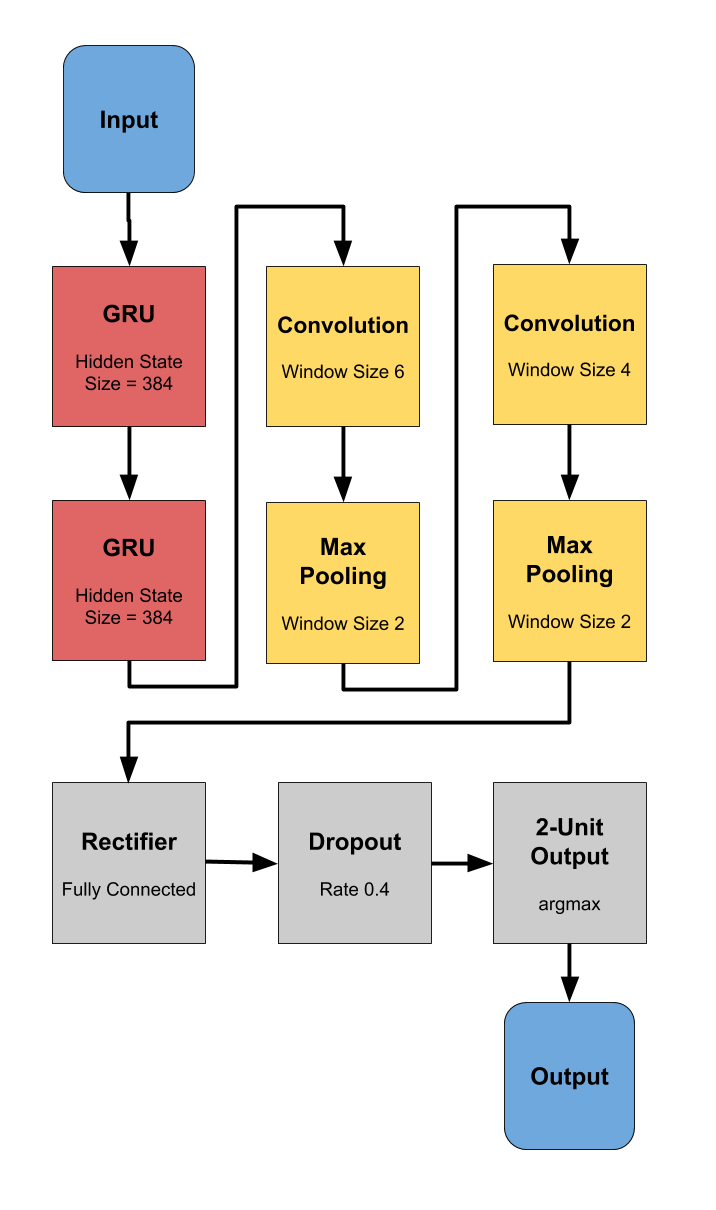
\includegraphics[scale=0.35]{our_model_architecture.png}
  \caption{Our Model}
  \label{fig:ourmodel}
\end{figure}

We trained the model for four epochs. Loss was calculated with sparse softmax cross
entropy with logits and an Adam optimizer was used for learning with clipped
gradient at 10 (to avoid instabilities; see Exploding Gradients
Problem\footnote{\url{https://machinelearningmastery.com/exploding-gradients-in-neural-networks/}})
and a learning rate of $10^{-4}$. Training on the Leonhard cluster took around
three hours.

This model achieved an accuracy of 87.4\% with the initial half of the test set,
which is a small improvement over the baseline B2.
The model achieved an accuracy of 86.6\% with the second/final half of the test set.

\section{Other Approaches} \label{sec:other}

The model described in \autoref{subsec:our-model} significantly outperforms
the random forest classifier described in \autoref{subsec:b1} and improves
slightly upon the plain RNN approach in \autoref{subsec:b2}. In addition to
these, we experimented with various other approaches.
However, no additional improvements could be achieved with
any of these creative methods.

\subsection*{Effect of word order}

In particular, we were interested in exploring the tradeoff between
increasing the amount of information encoded in each input (e.g. bag
of words vs embedding matrix) and the additional noise invited by
doing so. For example, even though it would seem that a sophisticated
model like the RNN used in \autoref{subsec:b2} and \autoref{subsec:our-model}
should benefit from more information (word order, context) this is only true
in practice assuming sufficiently large datasets and computational
resources \pisch{TODO not fully clear to me; is there a ref. for this reasoning?}.

It was our suspicion that weighing words independently had a much
stronger effect on classification performance than respecting
different word orders. Therefore we re-trained the RNN model presented
in \autoref{subsec:b2} again, but modified the pre-processing steps. Instead
of providing each tweet's embedding matrix as is, we sorted the
columns by vector norm. The idea was to normalize word order, while
still preserving the ability to assign individual weights to
words.
\pisch{TODO might it be helpful to describe this as a transformation of a
seq2seq model as used in classic RNN into a bag-of-words model?
just a thought}


\pisch{I do not agree with this conclusion. This result is lower than
the result of our model with 87.4\%. thus bag of words performs
worse than keeping the seq. Or did I miss something?}
This model achieved an accuracy of 85.2\%, confirming our hypothesis
that word order was not a significant contributor to accuracy, but
disproving the theory that respecting word order would add too much
noise for the RNN to handle.


\subsection*{Detecting negation}

We also tried to identify words within the scope of a negation using
the \texttt{nltk.sentiment.util.mark\_negation()} method from
NLTK\footnote{\url{https://www.nltk.org/}}.
Embedding vectors of negated words would then be multiplied by $-1.0$ before
feeding them into the RNN. Although detecting negation scopes and even
simple cases of double negation seemed to work very robustly, the
resulting model had a bit a lower accuracy than chosen final model presented in
\autoref{subsec:our-model}: 86.7\%. On the other hand, this result underlines
the power of the LSTM/GRU cells iniside the RNN, which seem to be able
to keep track of negation scopes automatically.


\subsection*{Additional training of the GloVe vectors}

For most models, we used the pre-trained 200 dimensional GloVe embeddings as
constants that were looked up within the tensorflow model. We tested additional
training on these pre-trained embeddings. Due to memory limitations of the GPU on
Leonhard, we could only use 100 dimensional GloVe embeddings for that test, which
did not improve the accuracy with the first half of the test set.


\subsection*{Additional embeddings}

Finally, we also tested additional embeddings.
We considered the remaining emojis in the tweets of particular interest.
Thus, we created an additional embedding vector that encoded the counts of the
known emojis \pisch{TODO are there any references for this?; any more description needed/desired here?}.

Additionally, we tested whether sentiment classification using lexicons of known 
positive and negative words could be used to improve our classifier.
Basically a difference value was calculated from the count of positive words in a 
tweet minus the count of negative words. Defined words like "not" were used to 
invert this value.\footnote{A more extended version of this additional Python code 
written by the same author (PS) had been used in his NLU group project 2 as 
described there. For this project here, no n-grams were built for multiple 
sentences, of course. Only the plain score for each tweet was used.} This concept 
follows the ideas described in the paper of Chaturvedi et al. 
2017~\cite{chaturvedi2017} and the available source code~\cite{chaturvedi_code}.

We tested both additional embeddings in various variants whether they could improve 
the accuracy of the model. First, we tested them as additional inputs of a final NN 
that took the results of baseline 2 model and these additional small embedding 
vectors to get the final 2 sentiment nodes. \texttt{argmax} for prediction, loss,
and optimizing functions for training were used identically as defined above.

Second, we tested these two additional embeddings in a small one layer NN to
generate a non-zero initial hidden state for the RNN. The rest of the model was 
identical to baseline 2. Here, the idea was tested whether such key information 
could be used to train relevant biases to the afterwards running RNN similar to the 
human brain that may take such key words as a first bias/primer when reading the 
entire tweet.

Despite theoretical considerations and despite the added complexity, both variants 
did not improve the accuracy of the models over the baseline B2.


\section{Conclusions}

Overall our additions do improve on the simple RNN baseline
established in \autoref{subsec:b2}, but not by much. Both RNN models do
however improve significantly on the random forest classifier. This
could hint at the strength and relative ease of an approach based on
taking short-term memory into account.

% pisch: I think this part is better removed. OK?
%Further investigation is
%neccessary to determine, whether the improvements are due to the GRU
%units or simply a result of the more powerful input model (sequence of
%word embeddings instead of a simple bag of words).

Despite testing various additional published and creative methods in addition,
we could not improve accuracy over the chosen final model.

A drawback of the more complex model (with respect to the relatively
small increase in accuracy) is the increased amount of available hyper-parameters
that can be tuned in the model, such as stack size,
convolution and pooling window sizes, stride lengths, dropout rate,
activation functions, etc. These hyper-parameters would have to be empirically
determined (via a grid search, for example). In combination with the
computational resources required to train the model, this makes it
 harder to further improve the model in a structured way.

\section*{Acknowledgements}

The authors wish to express their gratitude to the Euler and Leonhard
clusters at ETH, without whose unwavering computational effort this
project could not have been done.

\bibliographystyle{IEEEtran}
\bibliography{TheOptimists-literature}
\end{document}
